\chapter{输入/输出流简介}
现在来到泛讲篇的最后一章,让我们来看一下输入/输出流的相关知识。\par
一个基本的冯·诺依曼结构\footnote{冯·诺依曼结构(Von Neumann architecture),是一种存储程序逻辑架构。当今的主流计算机几乎都是依托于冯·诺依曼结构的。}计算机包含五个部分:控制器、运算器、存储器、输入设备和输出设备。
\begin{figure}[htbp]
    \centering
    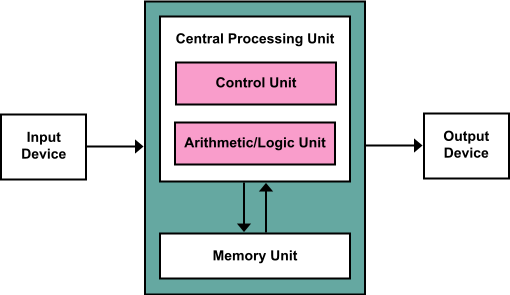
\includegraphics[width=.5\textwidth]{../images/generalized_parts/13_von_neumann_architecture.png}
    \caption{冯·诺依曼结构示意图}
\end{figure}
其中,输入设备和输出设备是计算机与外界进行交互的渠道。我们点击一个按扭,或者键入一串数字,或是扫描,或是摄像,甚至用蓝牙等传入信息,都是输入;电脑显示屏的显示内容,音乐的播放,文本的打印,都是输出。不过对于一个命令行界面的程序来说,用户与计算机的交互方式就很简单了。用户输入字符,程序显示字符,这是我们长期以来使用的交互方法。在本章,我们将进一步理解标准输入和输出,及它们的应用,并学习另外两种常用的输入输出方式。\par
\import{../generalized_parts/13_input_output_streams_overview/}{01_data_transfer_in_streams.tex}
\import{../generalized_parts/13_input_output_streams_overview/}{02_iostream.tex}
\import{../generalized_parts/13_input_output_streams_overview/}{03_sstream.tex}
\import{../generalized_parts/13_input_output_streams_overview/}{04_fstream.tex}
